\documentclass[holdfloat]{MSC-TESO-01}
\usepackage{graphicx}
\usepackage{amsmath}
\usepackage{relsize}
\usepackage{amsfonts}
\usepackage[english,spanish]{babel}
\usepackage{tikz}
\usetikzlibrary{shapes.geometric, arrows}

\usepackage{pgfplots}
\pgfplotsset{compat=1.14}
\usepackage{subcaption}

\usepackage{listings} 
\lstset{
     basicstyle=\fontsize{10}{10}\selectfont,
     keywordstyle=\color{blue}
}

\graphicspath{{images/}{chapter02/images/}{chapter03/images/}{chapter04/images/}}

\bibliographystyle{IEEEtran}


% ---------------------------------------------------
% Begin of Document
% ---------------------------------------------------

\begin{document}
\sloppy
\setlength{\baselineskip}{1\baselineskip}
\selectlanguage{Spanish}
% Information of the CsM student
\author{José Luis Magaña Vázquez}
%\cvu{000000}
\director{Dr. José Francisco Cervantes Álvarez}
%\director{Mtro. Luis Eduardo Pérez Bernal}
\title{DESARROLLO DE UN MÓDULO DE VISIÓN COMPUTACIONAL PARA VEHÍCULOS AEREOS NO TRIPULADOS UTILIZANDO DEEP LEARNING}
%\title{Recognition of Plant Diseases Using Convolutional Neural Networks}
\FechaDocumento{2 de marzo de 2020}
% Iteso shield
\itesoshield{images/iteso.png}
\maketitle
%: -----------------------------------------------
\fancypagestyle{plain}

%\include{acknowledgements}  
%\include{agradecimientos}
%\include{dedication}
%\include{dedicatoria}
%\include{abstract}
%\include{resumen}

%: ----------------------- Table of contents ------------------------

\setcounter{secnumdepth}{2} % organisational level that receives a numbers
\setcounter{tocdepth}{2}    % print table of contents for level 2
\tableofcontents            % print the table of contents
% levels are: 0 - chapter, 1 - section, 2 - subsection, 3 - subsubsection

%: ----------------------- list of figures/tables ------------------------

\listoffigures	% print list of figures

\listoftables  % print list of tables


\mainmatterSU

\chapter{Introducción}

\section{Título de la primer sección}
\section{Notación}
\begin{tabular}{|c|c|}
%\hline = horizontal borders
\hline
$\mathbf{A}$ & matriz \\
\hline
$A_{i,j}$ & elemento \textit{(i,j)} de \textbf{A} \\
\hline
$\mathbf{x},\mathbf{v},\mathbf{w}$ & vectores \\
\hline
$x_i, v_i. w_i$ & elemnto \textit{i}th de un vector \\
\hline
$\mathbf{w}^{(t)}$ & vector \textit{t} de un conjunto de vectores \\
\hline
$w_i^{(t)}$ & elmento \textit{i}th del vector $\mathbf{w}^{(t)}$ \\
\hline
\end{tabular}

\chapter{Estado del arte}
\textit{\textbf{Resumen:} La clasificación y detección de objetos es un importante campo dentro de la visión computacional, en los últimos años las redes neuronales convolucionales se han ganado el lugar en este campo al tener un buen desempeño en competencias y en las aplicaciones que necesitan aprendizaje que sería muy complicado si se deseara crear un algoritmo con reglas manuales, se presenta una breve recopilación de trabajos de interés dentro de las redes neuronales convolucionales}

\section{Clasificación}
Dentro de los algoritmos de clasificación de imágenes de redes neuronales se encuentran varios trabajos que han llevado al estado del arte hoy en día, a continuación se presentan algunos de relevancia debido a los conceptos y novedades que ha agregado al campo de la clasificación y locaclización usando redes neuronales.

\subsection{Aprendizaje basado en gradiente descendiente aplicado al reconocimiento de documentos - LeCun}
En éste artículo se nos muestra que dada una apropiada arquitectura de red neuronal, los algortimos de aprendizaje basados en el gradiente descendiente pueden ser usados para sintetizar un clasificador, tal como se muestra en su artículo, la red presentada apoya para la clasificación de caráteres escritos.
La red utilizada, es una red neuronal convolucional las cuales tienen un gran desempeño en clasificación de imágenes. La arquitectura de la red neuronal convolucional presentada se le llama LeNet-5 que consta de 3 capas convolucionales, 2 capas de muestreo y 2 capas completamente conectadas. El método usado para la actualización de los parámetros es el método de gradiente descendiente estocástico.
Durante el desarrollo del proyecto se utilizara el tipo de arquitectura de red convolucional para la clasificación de los objetos de interés, así como se aplicarán ciertas modificaciones de artículos más recientes.

\subsection{Clasificación ImageNet con redes neuronales convolucionales profundas - Krizhevsky}
En este artículo Krizhevsky presenta con una red nueronal convolucional tal y como lo hace LeCun, la aportación de este trabajo es la introducción de un método de regularización para prevenir el sobre ajuste de la red, este método de regularización es llamado "dropout". Este método consiste en forzar el valor a 0 a las neuronas en capas ocultas con una probabilidad de 0.5. De ese modo dichas neuronas no contribuyen a la clasificación haciendo que el entrenamiento no dependa de las mismas neuronas para realizar la clasificación y por lo tanto obliga a la red a aprender caractisticas de manera más robusta. De esta manera se evita el sobre ajuste pero el costo es que se requiere mayor cantidad de entrenamiento para que la red neuronal converja.
Durante el trabajo utilizaremos técnicas de normalización como el presentado por Krizhevsky, para evitar el sobre ajuste.

\subsection{Red en Red - Lin}
En el atículo presentado por Lin et al, se introduce una modificación a la red neuronal convolucional. En la capa de convolución normalmente se utilizan kernel locales para obtener los mapas de carecterísticas, en su lugar en éste trabajo se propone reemplazarlo por una red neuronal basados en el perceptrón, para ser el responsable de obtener los mapas de caracteríscas. Además agrega un método de regularización llamado "Global average pooling" o muestreo promedio global el cual toma el promedio de cada mapa de características el cuál se pasa a una capa "softmax", con cual los autores describen que refuerza las correspondencias entre los mapas de características y categorías, y es más robusto en translaciones espaciales del objeto de interés.

\subsection{Redes convolucionales muy profundas para reconocimiento de imágenes a grande escala - Simonyan}
Hasta ahora en los trabajos se han introducido cambios en las capas de convolución, pero qué tal aumentar o disminuir la profundidade de la red. En cuanto al manejo de la profundidad de la red neuronal, Simonyan y Andrew presentaron en su artículo el efecto de hacer redes más profundas y su precisión al modificarlas, con profundidad de hasta 19 capas, en su investigación arrojaron que se puede aumentar la precisión haciendo más profunda la red logrando tener buenos resultados y disminuyendo la dimensión de filtros convolucionales o kernels locales, en este caso de dimensión 3x3.

\subsection{Aprendizeje residual profundo para reconocimiento de imágenes - He}
Siguiendo con los trabajos que experimentan con redes neuronales más profundas, He et al, que expone que diseñar redes neuronales muy profundas lleva a una degradación durante el entrenamiento donde la precisión se satura y comienza un degradamiento. Como parte de enfrentar este comportamiento, He et al, introducen un nuevo tipo de bloque a las redes neuronales llamado aprendizaje residual, el cual se tienen dos capas, la primera capa procesa normalmente la información de entrada, pero la segunda capa, toma como entrada, los datos de salida de la primera capa más los datos de entrada de la primera capa. Con esto se muestra que pueden diseñar redes con mayor porfundidad y manejando el degradamiento que habían observado con las redes neuronals habituales. Con este tipo de bloque en la red neuronal, experimentaron con profundidades de hasta 152 capas a diferencia de las 19 capas usadas por Simonyan, este tipo de red se llamó ResNet.

\subsection{Iendo profundo con convoluciones - Szegedy}
En este trabajo Szegedy et al, introducen un nueva arquitectura llamada "Inception", esta arquitectura se basa en un modulo de "inception", en este modulo todos los kernels son aprendidos y que es un conjunto de filtros de diferentes dimensiones que procesan la entrada y al final se combinan como preparación para el siguiente módulo de "inception".

\section{Localización y clasificación}
Como parte de los problemas relacionados en la visión computacional, el problema que se aborda en este proyecto no solo es la clasificación sino también la localización del objetos dentro de la imagen. Existen varias implementaciones para abordar estas tareas en conjunto.

\subsection{Solo observas una vez: Unificado, detección de objetos en tiempo real - Redmon}
Parte del manejo de imágenes no solamente es la clasificación sino también la localización en un imagen de varios elementos de interes. En este trabajo Redmon et al, presenta una arquitectura que diferente a lo que se había hecho en trabajos previos donde la detección de objetos se han dividido en dos etapas, la localización y la clasificación. Redmon et al, propone una sola etapa en su arquitectura YOLO. Arquitecturas previas parten la imagen en varias regiones, donde genera cuadros delimitadores potenciales para ejecutar la clasificación sobre estas cajas protenciales. Al final un post procesamiento es realizado para refinar los cuadros delimitadores, eliminar duplicados de imagen y generar las clasificaciones finales.
YOLO predice simultaneamente multiples cajas delimitadoras y clases de probabilidad de cada una. Esta arquitectura es entrenada para en imagenes completas para la optimización. Por lo que aprende del objeto de interés y su contexto, lo que lo lleva a generar menos falsos en imagenes que no son de interés. En contra tiene que al generar menos cajas delimitadoras y tiene un límite de predicciónes por cada una, va por detrás de otros modelos en la detección de objetos pequeños.
\chapter{Marco Teórico Conceptual}


\section{Aprendiendo a partir de datos}
Existen varios acercamientos de aprendizaje máquina automático, pero uno de los acercamientos más exitosos ha sido el llamado aprendizaje basado en el gradiente. El modelo de aprendizaje calcula una función $Y^p=F\left(Z^p,W\right)$[3] donde $Z^p$ es la p-th patrón de entrada, $W$ representa la colección de parámetros ajustables en el sistema y  $Y^p$ puede ser interpretada como la etiqueta o clase del patrón $Z^p$, o la probabilidad asociada a cada clase a predecir. Es decir que a partir de una entrada se predice la clasificación deseada por medio de una función F.

$E^p=D\left(D^p,F\left(Z^p,W\right)\right)$ [3], es una función que mide la discrepancia o error entre $D^p$ el cuál es el valor correcto que deseamos predecir a partir del patrón de entrada $X^p$ y la predicción $Y^p$. Esto implica tener una base de datos con los patrones de entrada con su respectiva salida correcta para poder realizar esta operación con la cuál se entrena el modelo. Con el cálculo del error de cada predicción se puede calcular el promedio y obtener un error de entrenamiento $E_{train}\left(W\right)$ que se llamará función de costo o pérdida. Así muchos algoritmos de aprendizaje tratan de minimizar $E\left(W\right)$. 


\section{Gradiente descenciente}
El algoritmo de gradiente descendiente intenta minimizar la función de costo $E\left(W\right)$ a través de variaciones en los pesos $W$. Estas variaciones son introducidas a cada peso partir del gradiente de la función de perdida con respecto a los pesos. Pero para ello se tiene que cumplir que los parámetros de W son valores reales para los cual la función de costo es una función continua y diferenciable, de esta manera se introducen variaciones en cada parámetro de W iterativamente de la siguiente forma:
$W_k=W_{k-1}-\epsilon\frac{\partial E\left(W\right)}{\partial W}$[3]
Existen variaciones del gradiente descendiente siendo el presentado uno de los más simples.

\section{Perceptrón}
El perceptrón es un modelo computacional de una neurona[4], donde una sola neurona tiene varias entradas (dentritas), un cuerpo celular y una salida (axón). Replicando esto el perceptrón tiene varias entradas y una sola salida, el cuál consiste en un vector de “pesos” w = [w1 … wm], un peso para cada entrada más un “bias” o tendencia cuyo parámetro es descrito como b.
Con los parámetros dados w y b el perceptrón realiza el siguiente cálculo:
$$f\left(x\right)=1\ \ \ \ \ \ \ \ \ \ \ \ if\ b+\sum_{i=1}^{l}{x_iw_i}>0$$
$$f\left(x\right)=0\ \ \ \ \ \ \ \ \ \ \ \ \ \ \ de\ otra\ manera$$
Donde $f\left(x\right)$ se llama función de activación.
El algoritmo del perceptrón busca obtener o aprender los pesos w tales que dados los datos de cada ejemplo de entrenamiento $x^k=\left[x_1^k ... x_j^k\right]$, se obtenga la correcta clasificación binaria $a^k$, donde $a^k$ será 1 o 0 en este caso. 
\begin{figure}[htbp]
\begin{center}
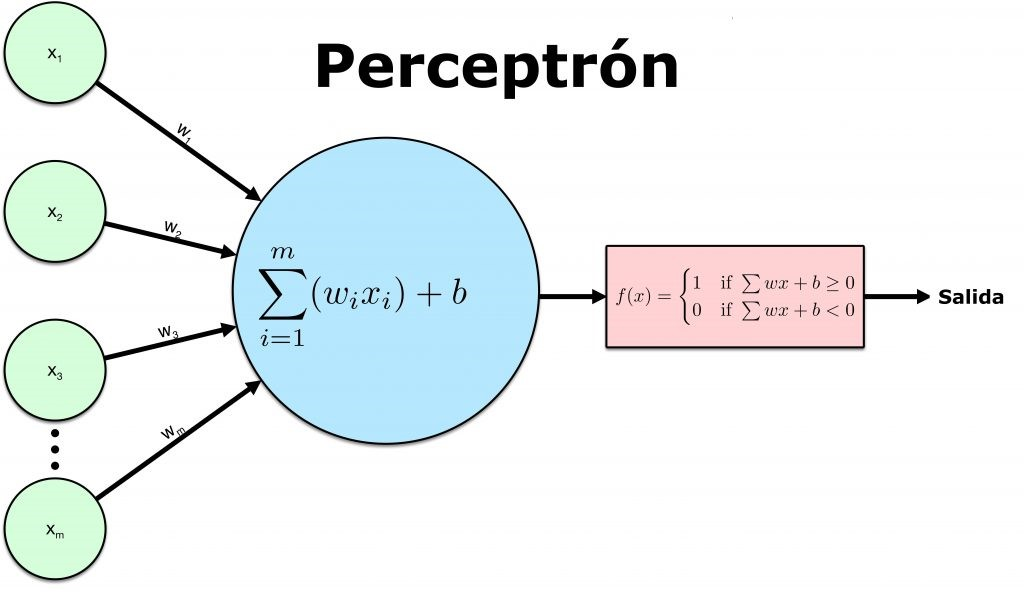
\includegraphics[width=3in]{capítulo3/Perceptron.jpg}
%http://blog.josemarianoalvarez.com/2018/06/10/el-perceptron-como-neurona-artificial/
\caption{Modelo del perceptrón}
\label{fig:perceptron}
\end{center}
\end{figure}
A continuación, se presenta el algoritmo del perceptrón[4]:
\begin{enumerate}
    \item Inicializar los parámetros w y b
    \item Durante N iteraciones (definidas por el desarrollador) o hasta que los pesos no cambien realizar lo siguiente:
    \begin{enumerate}
        \item Para cada ejemplo de entrenamiento $x^k$ con respuesta $a^k$
             \begin{itemize}
                 \item Calcular $f\left(x^k\right)$
                 \item Si $a^k\ -\ f\left(x^k\right)\ =\ 0$  continua
                 \item Si no, actualizar todos los pesos como a continuación $$ w_i = w_i+\left(a^k-f\left(x^k\right)\right)x_i $$
             \end{itemize}
    \end{enumerate}
\end{enumerate}
Donde si existe una configuración de pesos w con los cuales se puedan clasificar correctamente cada elemento de entrenamiento, el algoritmo lo encontrará, aunque en ejemplos reales no siempre es posible, el algoritmo puede encontrar una configuración de pesos w para clasificar correctamente un porcentaje de los elementos de entrenamiento.
En casos donde se necesite más clases se puede realizar incrementando la cantidad de perceptrones por cada clase, siendo el valor 0 el indicador de no pertenencia a la clase y el número 1 la pertenencia a la clase, teniendo así una llamada red neuronal.
\section{Red Neuronal Clásica}
Cómo se ha visto con el perceptrón, una red neuronal clásica consiste en conjunto de modelos computacionales llamadas neuronas, las cuales tienen parámetros ajustables w y “bias” que, por medio de un algoritmo, la red puede aprender a clasificar correctamente las clases a partir de los datos de entrada $x^k$.
\begin{figure}[htbp]
\begin{center}
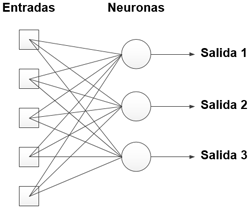
\includegraphics[width=3in]{capítulo3/RedNeuronalClasica.png}
%https://www.ediciones-eni.com/open/mediabook.aspx?idR=6d7e746f6a1fe07834a44f834c84d6ba
\caption{Modelo de una red neuronal de una sola capa}
\label{fig:rnc}
\end{center}
\end{figure}
En la Figura~\ref{fig:rnc} se puede observar un modelo de red neuronal, cuyas neuronas tienen una salida. Ahora, las salidas de las neuronas en la imagen podríamos tomarlas como entrada para un siguiente conjunto de neuronas, a cada conjunto de neuronas se les llama capas, siendo una capa las neuronas que reciben la entrada original, una segunda capa de neuronas como entrada la salida de la primera capa, teniendo una llamada red neuronal multicapa, donde a las capas entre la entrada y la salida se les llama capas ocultas como se presenta en la Figura~\ref{fig:rnc2}. 
De esta manera se pueden obtener redes neuronales de n capas, por lo que cada capa aumenta el tamaño o la “profundidad” de la red neuronal, y es aquí de donde procede el termino aprendizaje profundo o también conocido en inglés como “Deep learning”.
\begin{figure}[htbp]
\begin{center}
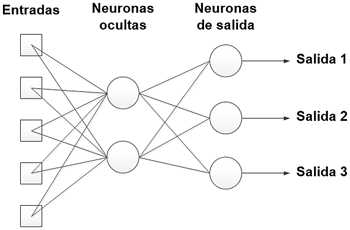
\includegraphics[width=3in]{capítulo3/RedNeuronalClasica2.png}
%https://www.ediciones-eni.com/open/mediabook.aspx?idR=dd1e7c64bbcc8628f67483605a21d1d2
\caption{Modelo de una red neuronal con una capa oculta}
\label{fig:rnc2}
\end{center}
\end{figure}
\section{Red Neuronal Feed Fordward y Back Propagation}
Son redes neuronales cuyo grafo con dirección no contienen ciclos, normalmente las redes neuronales multicapa utilizan un algoritmo de gradiente descendiente para calcular el valor de modificación de los pesos w, donde la diferencia de las neuronas del tipo perceptrón es el cambio de la función de activación, donde la función de activación del perceptrón está dada por:
$$f\left(\ x\right)=1\ \ \ \ \ \ \ \ \ \ \ \ if\ b+\sum_{i=1}^{l}{x_iw_i}>0$$
$$f\left(x\right)=0\ \ \ \ \ \ \ \ \ \ \ \ \ \ \ de\ otra\ manera$$
Esto debido que, para hacer uso del gradiente descendiente necesitamos que la función de costo o pérdida sea diferenciable y continua para el conjunto de valores reales de los pesos w. Dado que la función de pérdida $E^p=D\left(D^p,F\left(W,Z^p\right)\right)$[3] depende de la función de activación, la función del perceptrón no cumple los requisitos para implementar el gradiente descendiente.
Existen varias funciones de activación, una de las funciones usadas para las redes neuronales “feed forward” es la función sigmoide:
$$f\left(z\right)=\frac{1}{1+e^{-z}}$$
 La cual es derivable:
$$f^\prime\left(z\right)=f\left(z\right)\left(1-f\left(z\right)\right)$$
Donde 
$$z=\ b+\sum_{i=1}^{l}{x_iw_i}$$
Por lo cual se puede utilizar como función de activación y poder calcular el gradiente de la función de perdida para actualizar los pesos w. A dicho proceso con el cuál se calcula el gradiente a partir de la función de costo o pérdida y se actualizan los pesos w se le llama “back propagation”.

\section{Red Neuronal Convolucional}
Hasta ahora se ha considerado las redes neuronales completamente conectadas, pero estas también pueden ser parcialmente conectadas y un caso especial son las redes neuronales convolucionales, las cuales son muy recurridas es visión computacional.[4]
Las redes convolucionales combinan tres ideas para asegurar algún grado de invarianza en deslizamiento, escala y distorsión: campos receptivos locales, pesos compartidos y sub muestreo espacial o temporal. Los campos receptivos locales son llamados filtros o kernel, donde para una imagen en 2 dimensiones un filtro de dimensión 3x3, como ejemplo se podría ver de la siguiente forma:

$$\begin{matrix}a_1^1&a_1^2&a_1^3\\a_2^1&a_2^2&a_2^3\\a_3^1&a_3^2&a_3^3\\\end{matrix}$$

De una imagen de dimensión nxm se toma una parte de la dimensión del filtro viendo la parte superior izquierda como el punto de partida, y se realiza un producto punto, luego se toma de nuevo otra parte de la imagen de 3x3 pero esta vez tomamos los valores que están hacia la derecha desplazando la ventana un paso, uno en este caso y se realiza la misma operación con el filtro. Se repite la misma operación de desplazamiento y producto punto sobre toda la imagen, donde los valores resultantes dan otra imagen después de haber pasado por el filtro. Dicho filtro puede contener valores que “filtren” líneas verticales, horizontales, esquinas o puntos finales. Por lo que la imagen puede pasar por varios filtros obteniendo por cada filtro un mapa de característica y al final varios mapas con diferentes características. Esta capa de operaciones con filtros y desplazamiento se llama capa convolucional. Con este tipo de capa se busca que la red pueda aprender a partir de las características obtenidas por los filtros en lugar de los datos crudo de los pixeles.
Otra capa en una red convolucional es llamada “pooling” o de agrupación, que es un sub muestreo de la imagen de entrada para reducir sus dimensiones, la operación que realiza puede ser que a partir de una ventana por ejemplo de dimensión de 2x2 de la imagen de entrada y obtener el mayor valor que pasara a conformar la imagen reducida de salida, al finalizar el barrido sobre la imagen. Con este tipo de capa se busca reduciendo la sensibilidad de la red al desplazamiento y las distorsiones de la imagen entrada.
\begin{figure}[htbp]
\begin{center}
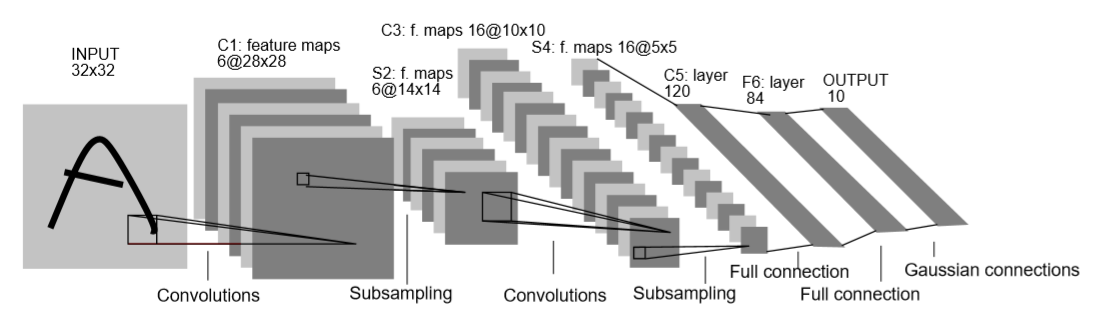
\includegraphics[width=4in]{capítulo3/LeNet.png}
%Y. LeCun, L. Bottou, Y. Bengio, y P. Haffner, «Gradient-Based Learning Applied to Doument Recognition», Proc. of the IEEE, November 18.
\caption{Modelo de una red neuronal con una capa oculta}
\label{fig:lenet}
\end{center}
\end{figure}
En la Figura~\ref{fig:lenet} se presenta un ejemplo de una red convolucional llamada LeNet-5 [3] en donde se puede observar 3 capas convolucionales C1, C3  y C5, dos capas de agrupación S2 y S4 y una capa completamente conectada.

%[1]	J. Schmidhuber, «Deep Learning in Neural Networks: An Overview», Neural Networks, vol. 61, pp. 85-117, ene. 2015, doi: 10.1016/j.neunet.2014.09.003.
%[2]	«ImageNet Large Scale Visual Recognition Competition (ILSVRC)». http://image-net.org/challenges/LSVRC/ (accedido oct. 07, 2019).
%[3]	Y. LeCun, L. Bottou, Y. Bengio, y P. Haffner, «Gradient-Based Learning Applied to Doument Recognition», Proc. of the IEEE, November 18.
%[4]	E. Charniak, Introduction to Deep Learning, 1st ed. The MIT Press, 2018.
%[5]	«Red neuronal artificial», Wikipedia, la enciclopedia libre. oct. 04, 2019, Accedido: oct. 06, 2019. [En línea]. Disponible en: https://es.wikipedia.org/w/index.php?title=Red_neuronal_artificial&oldid=119954405.
%[6]	V. E. Bondarenko, «Artificial neural networks», Salem Press Encyclopedia of Science. Salem Press, 2018.
%[7]	«t8neuronales.pdf». Accedido: oct. 06, 2019. [En línea]. Disponible en: http://www.sc.ehu.es/ccwbayes/docencia/mmcc/docs/t8neuronales.pdf.
%[8]	«Dialnet-ENTRENAMIENTODEUNAREDNEURONALARTIFICIALUSANDOELALG-4844874.pdf». .
%[9]	S. Shalev-Shwartz y S. Ben-David, Understanding Machine Learning from Theory to Algorithms. Cambridge University Press, 2015.

%\include{chapter04/chapter04}
%\include{chapter05/chapter05}
%\include{chapter06/chapter06}

\bibliography{biblio}

\end{document}
